\section{Liste des élements à installer}
\begin{itemize}
    \item Deux rails de leds IR.
    \item Un boitier étanche contenant: Le Rpi4, la caméra, le transformateur 12VDC-5VDC, le régulateur 1.5V, le jeu de relai et le fusible d'entrée.
    \item Tiroir pour la télécommande avec le jeu d'aimant de levage.
\end{itemize}
\section{Disposition prévue}
Comme indiqué dans le chapitre \ref{chap:exi}, nous avons possibilité d'utiliser le support perforé ainsi que la zone libre sur le timon.
Le principe est le suivant, fixer le boitier étanche à une plaque d'aluminium qui elle même sera fixer sur le support, ainsi, il sera plus simple
de placer le boitier selon les besoins.

La camera et son filtre seront placés dans le boitier et plaqués contre la facade transparente, de manière à observer la route entre le semoir
et le pick-up.

Les rails de leds IR seront placés de part et d'autre du timon à 80 \si{\centi\metre} du semoir en direction du pick-up pour "éclairer" le champ
de vue de la caméra. Dans l'idéal, al fixation permettra aux deux rails de se replier sur le timon lorsque l'éclairage ne sera pas utilisé,
cependant il n'est pas certain que ce sera effectué durant la période dédiée au TB.

Le tiroir permettant de contrôler la télécommande sera placé sur le boitier étanche, celui-ci s'ouvrant de face, ça ne posera pas problème.

Les illustations suivantes permettent de se faire une idée plus précise de ce qui est prévu.

\begin{figure}[H]
    \centering
    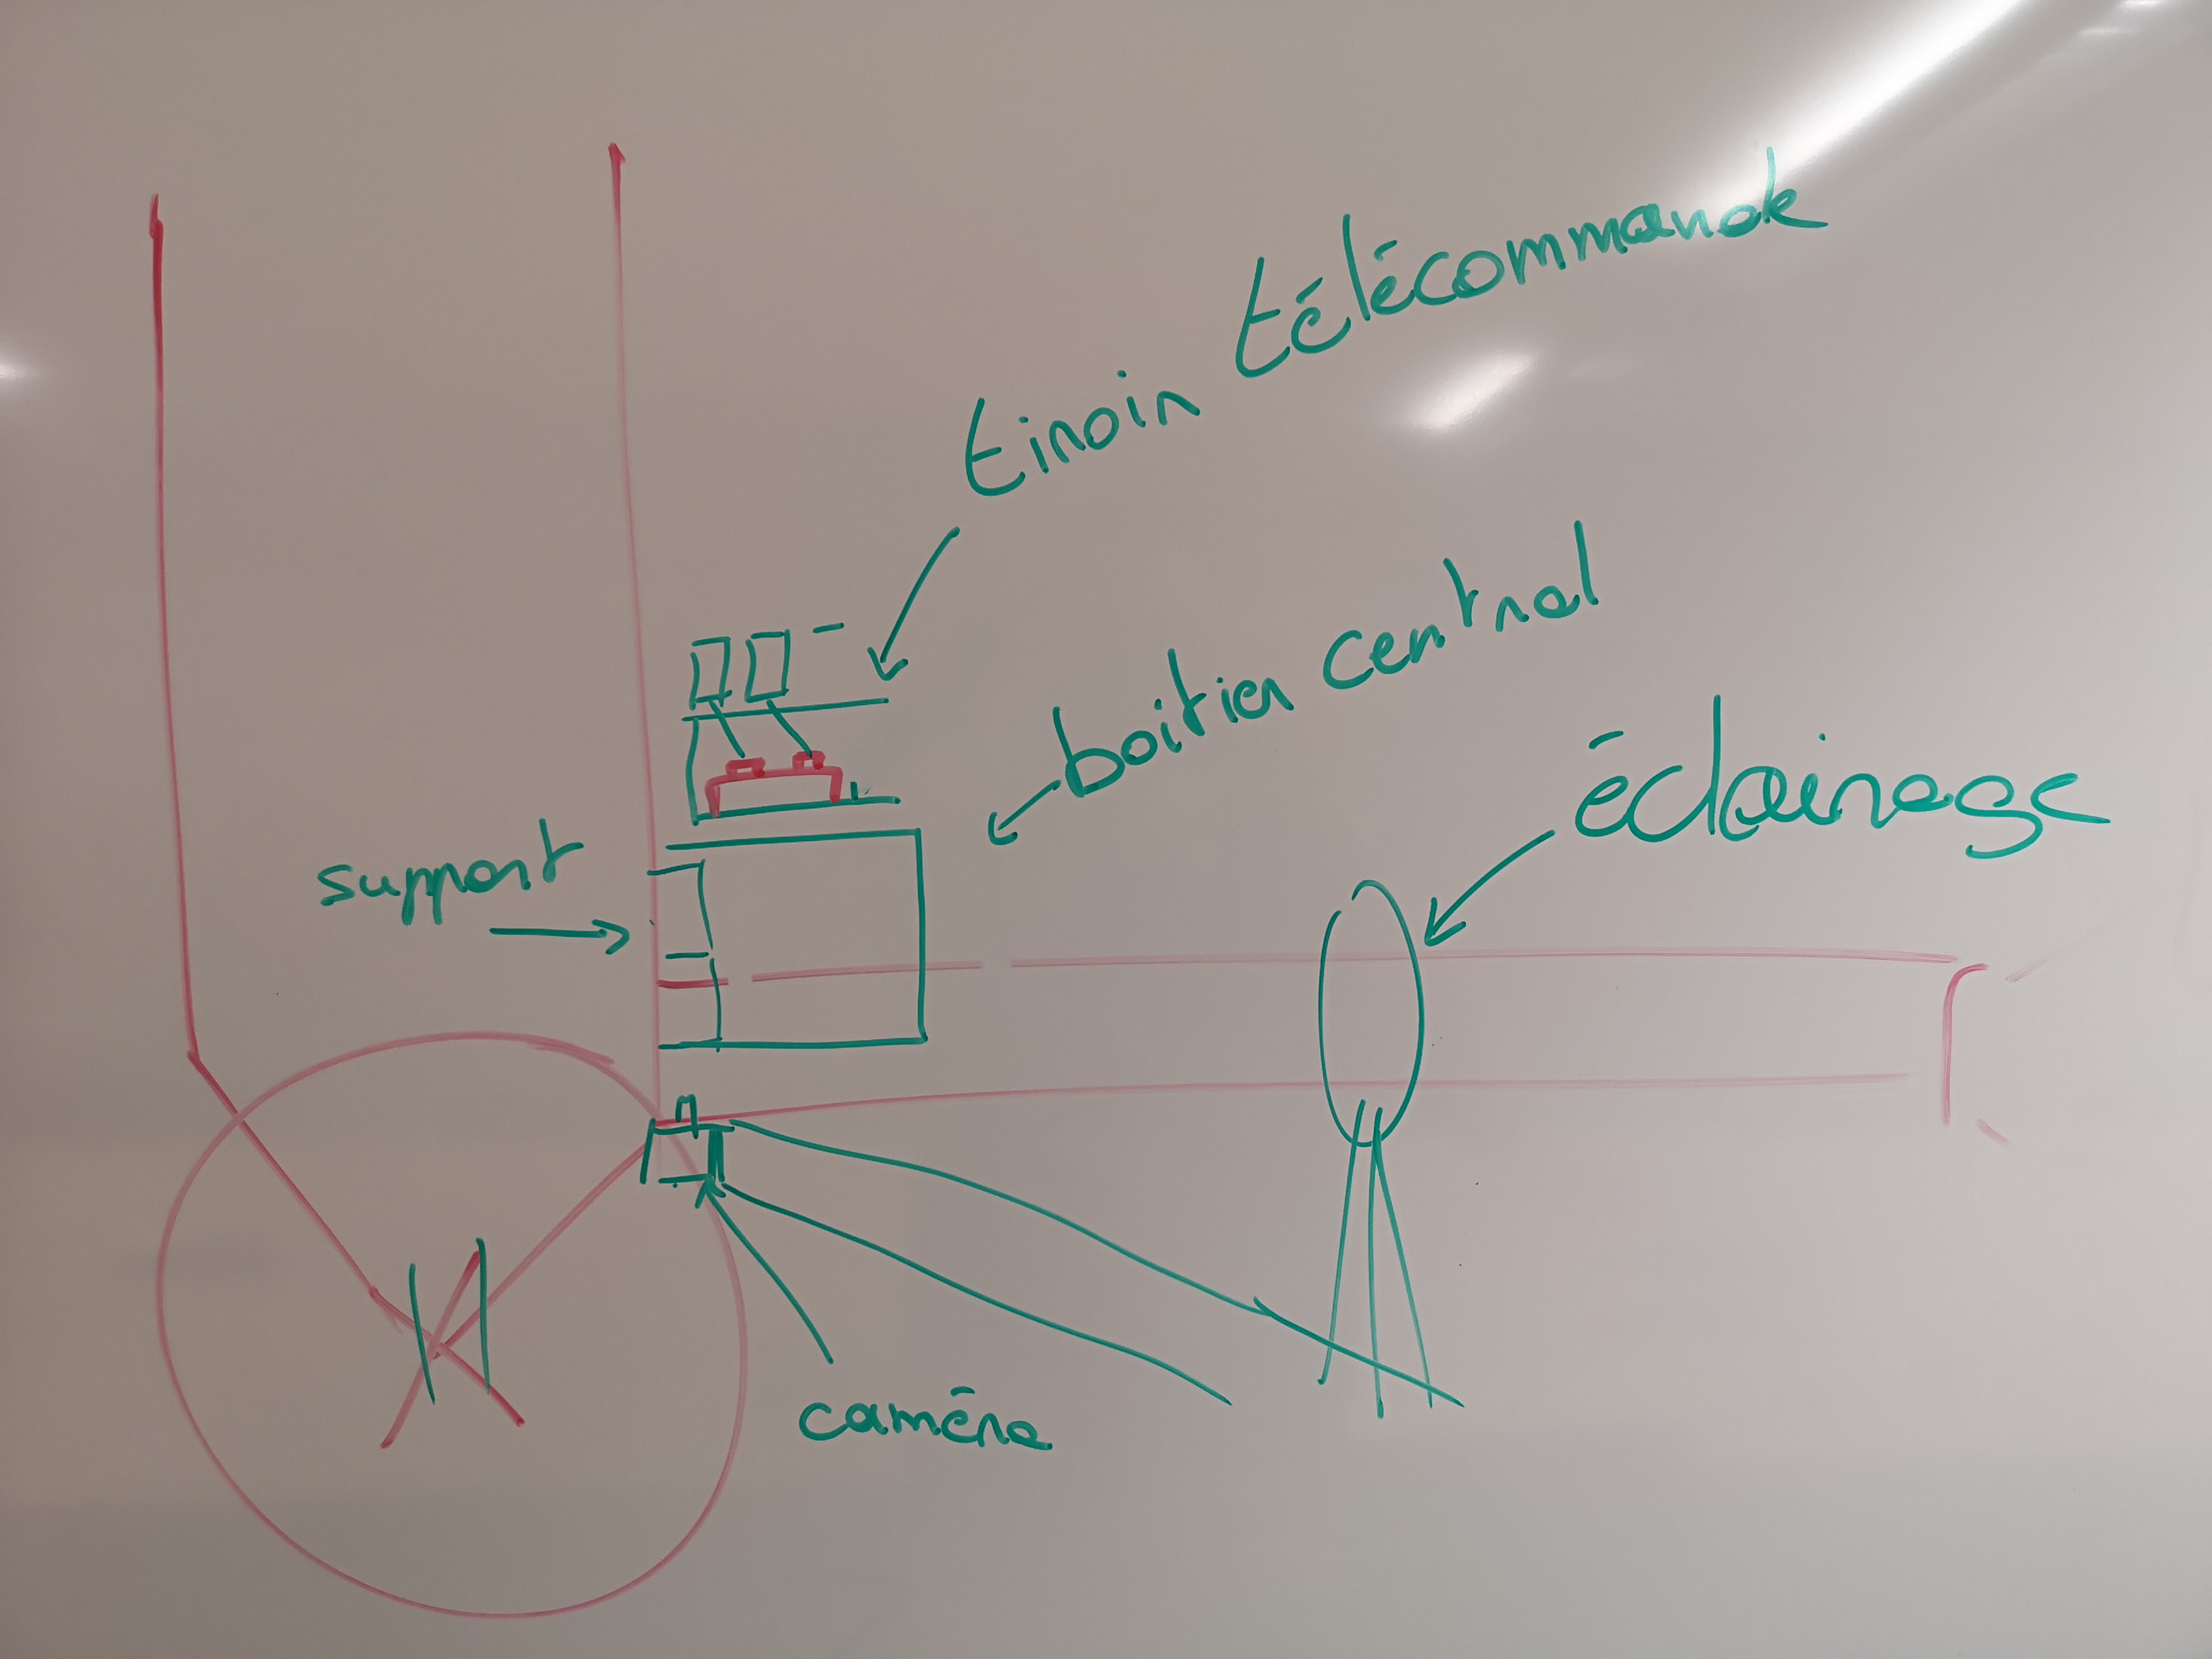
\includegraphics[height=7cm]{assets/figures/montage1.jpg}
    \caption{Montage prévu - Vue de côté}
\end{figure}

\begin{figure}[H]
    \centering
    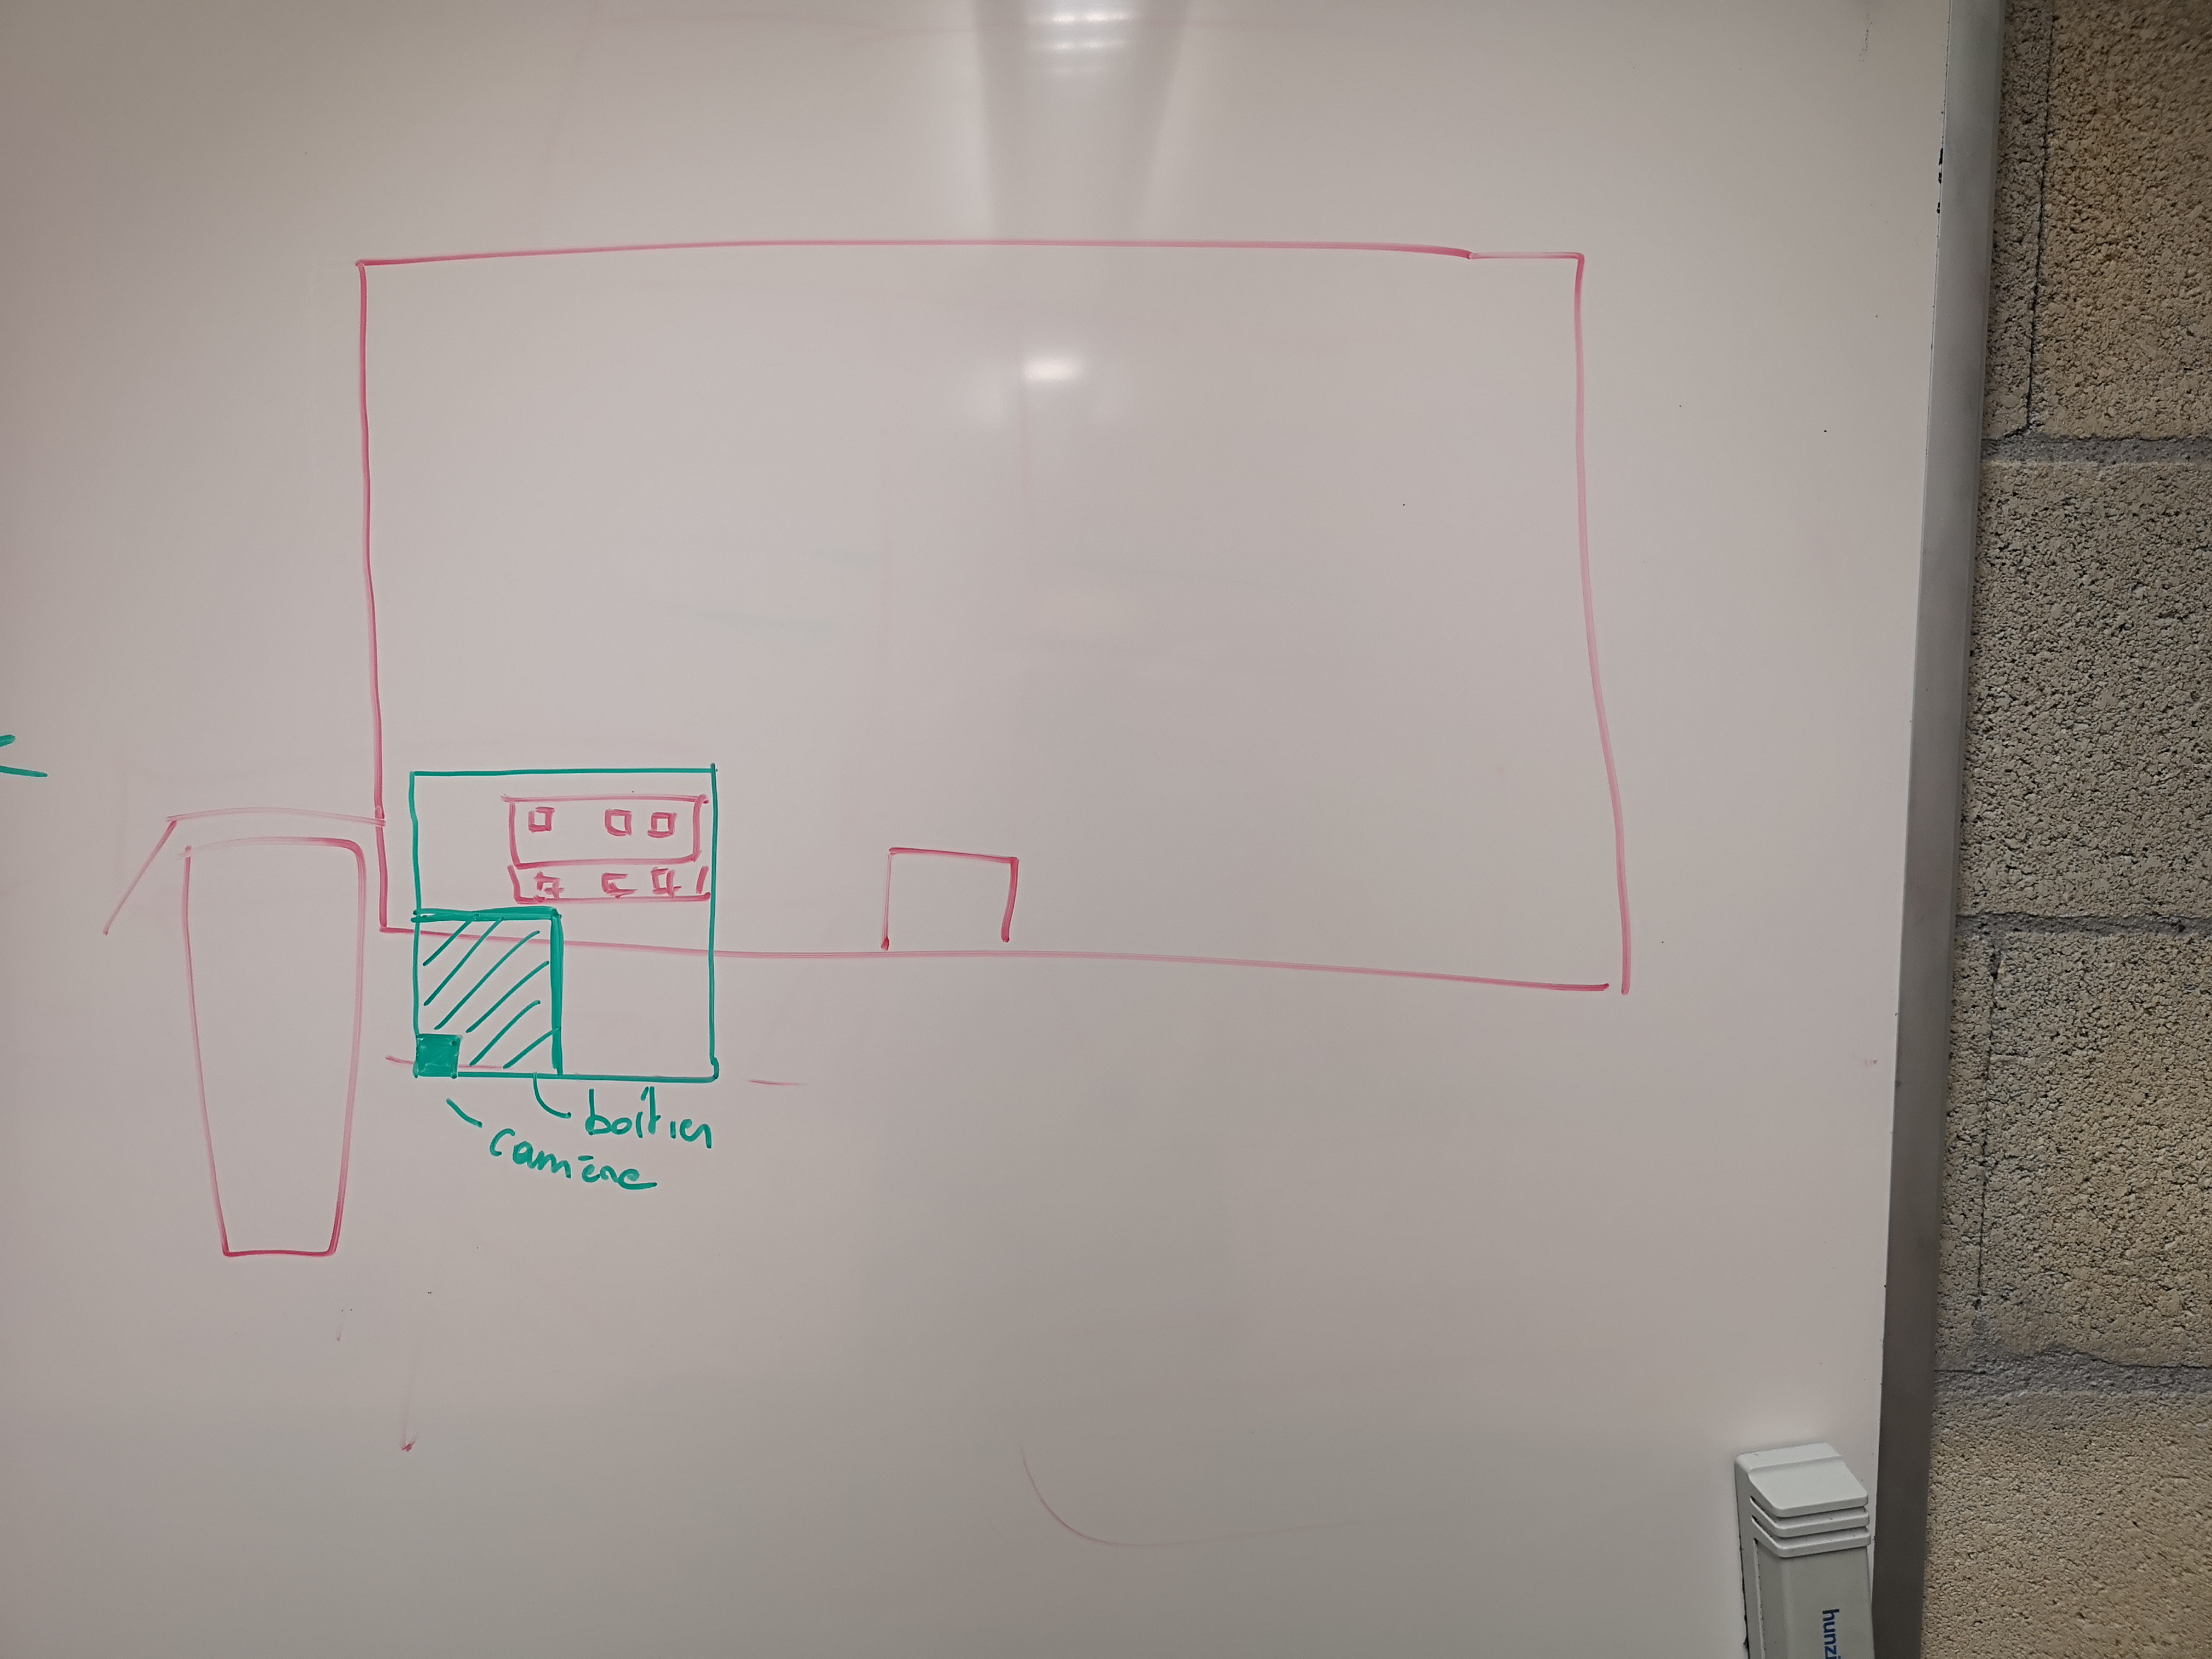
\includegraphics[height=7cm]{assets/figures/montage2.jpg}
    \caption{Montage prévu - Vue de face}
\end{figure}

\begin{figure}[H]
    \centering
    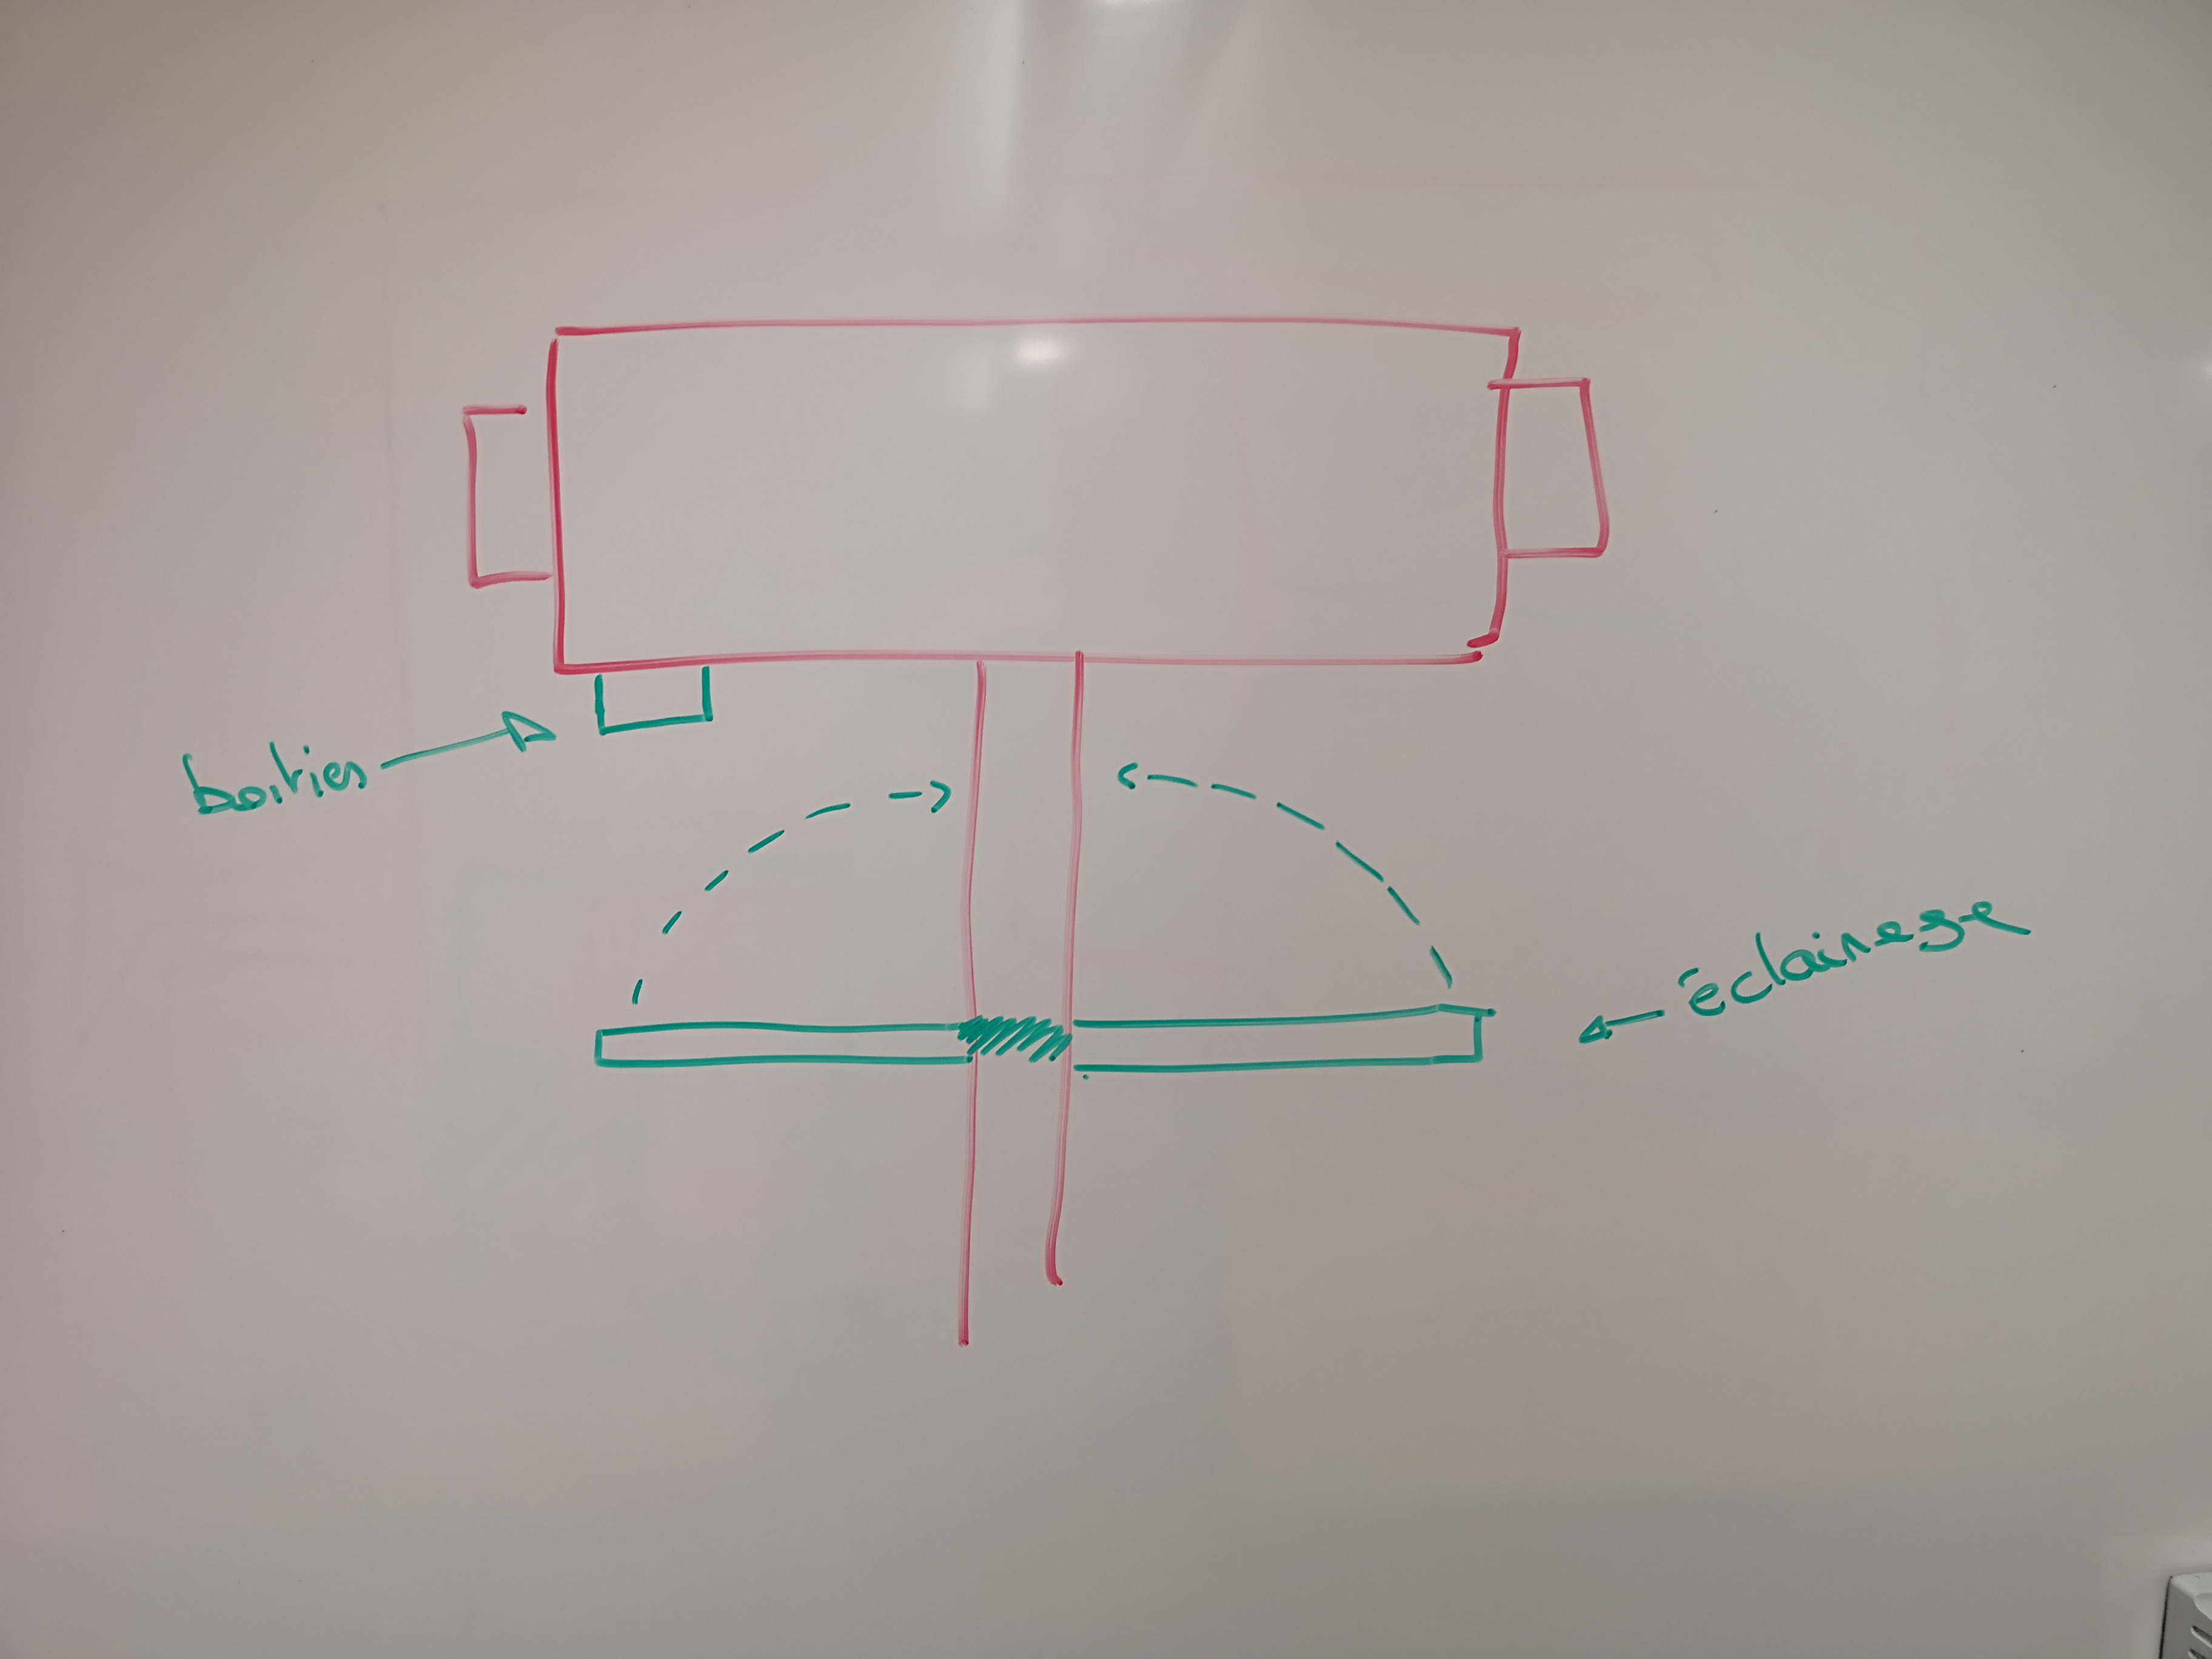
\includegraphics[height=7cm]{assets/figures/montage3.jpg}
    \caption{Montage prévu - Vue du dessus}
\end{figure}

[Ajouter quelque mots/illustration pour la mesure de vitesse]
\section{Installation réel}
\subsection{Eclairage}
Le timon ne pouvant pas être perçé, j'ai imaginé la fixation suivante pour le maintient des barres de leds.

\begin{figure}[H]
    \centering
    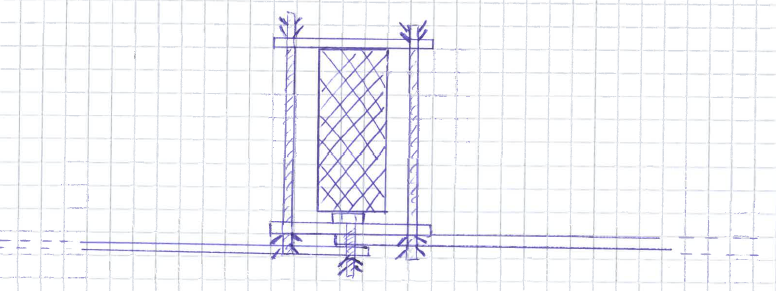
\includegraphics[width=13cm]{assets/figures/fixation_eclairage_face.PNG}
    \caption{Fixation leds - Vue de face}
\end{figure}

\begin{figure}[H]
    \centering
    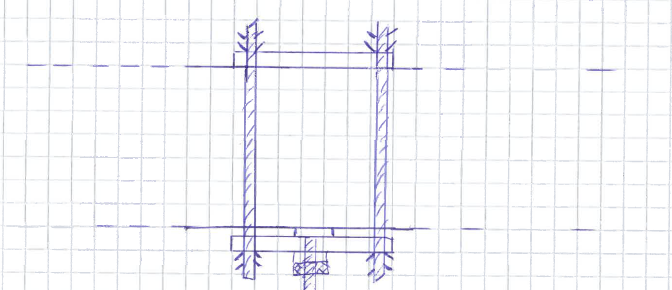
\includegraphics[width=13cm]{assets/figures/fixation_eclairage_cote.PNG}
    \caption{Fixation leds - Vue de côté}
\end{figure}

Le principe est de visser les deux rails à une première plaque en aluminium, puis visser celle-ci à une seconde plaque placée au dessus du timon,
de manière à le serrer. Cette solution ne permet pas de replier les leds, mais c'est suffisamment solide pour effectuer des tests de détection.

Ci-dessous, le montage réalisé:

\begin{figure}[H]
    \centering
    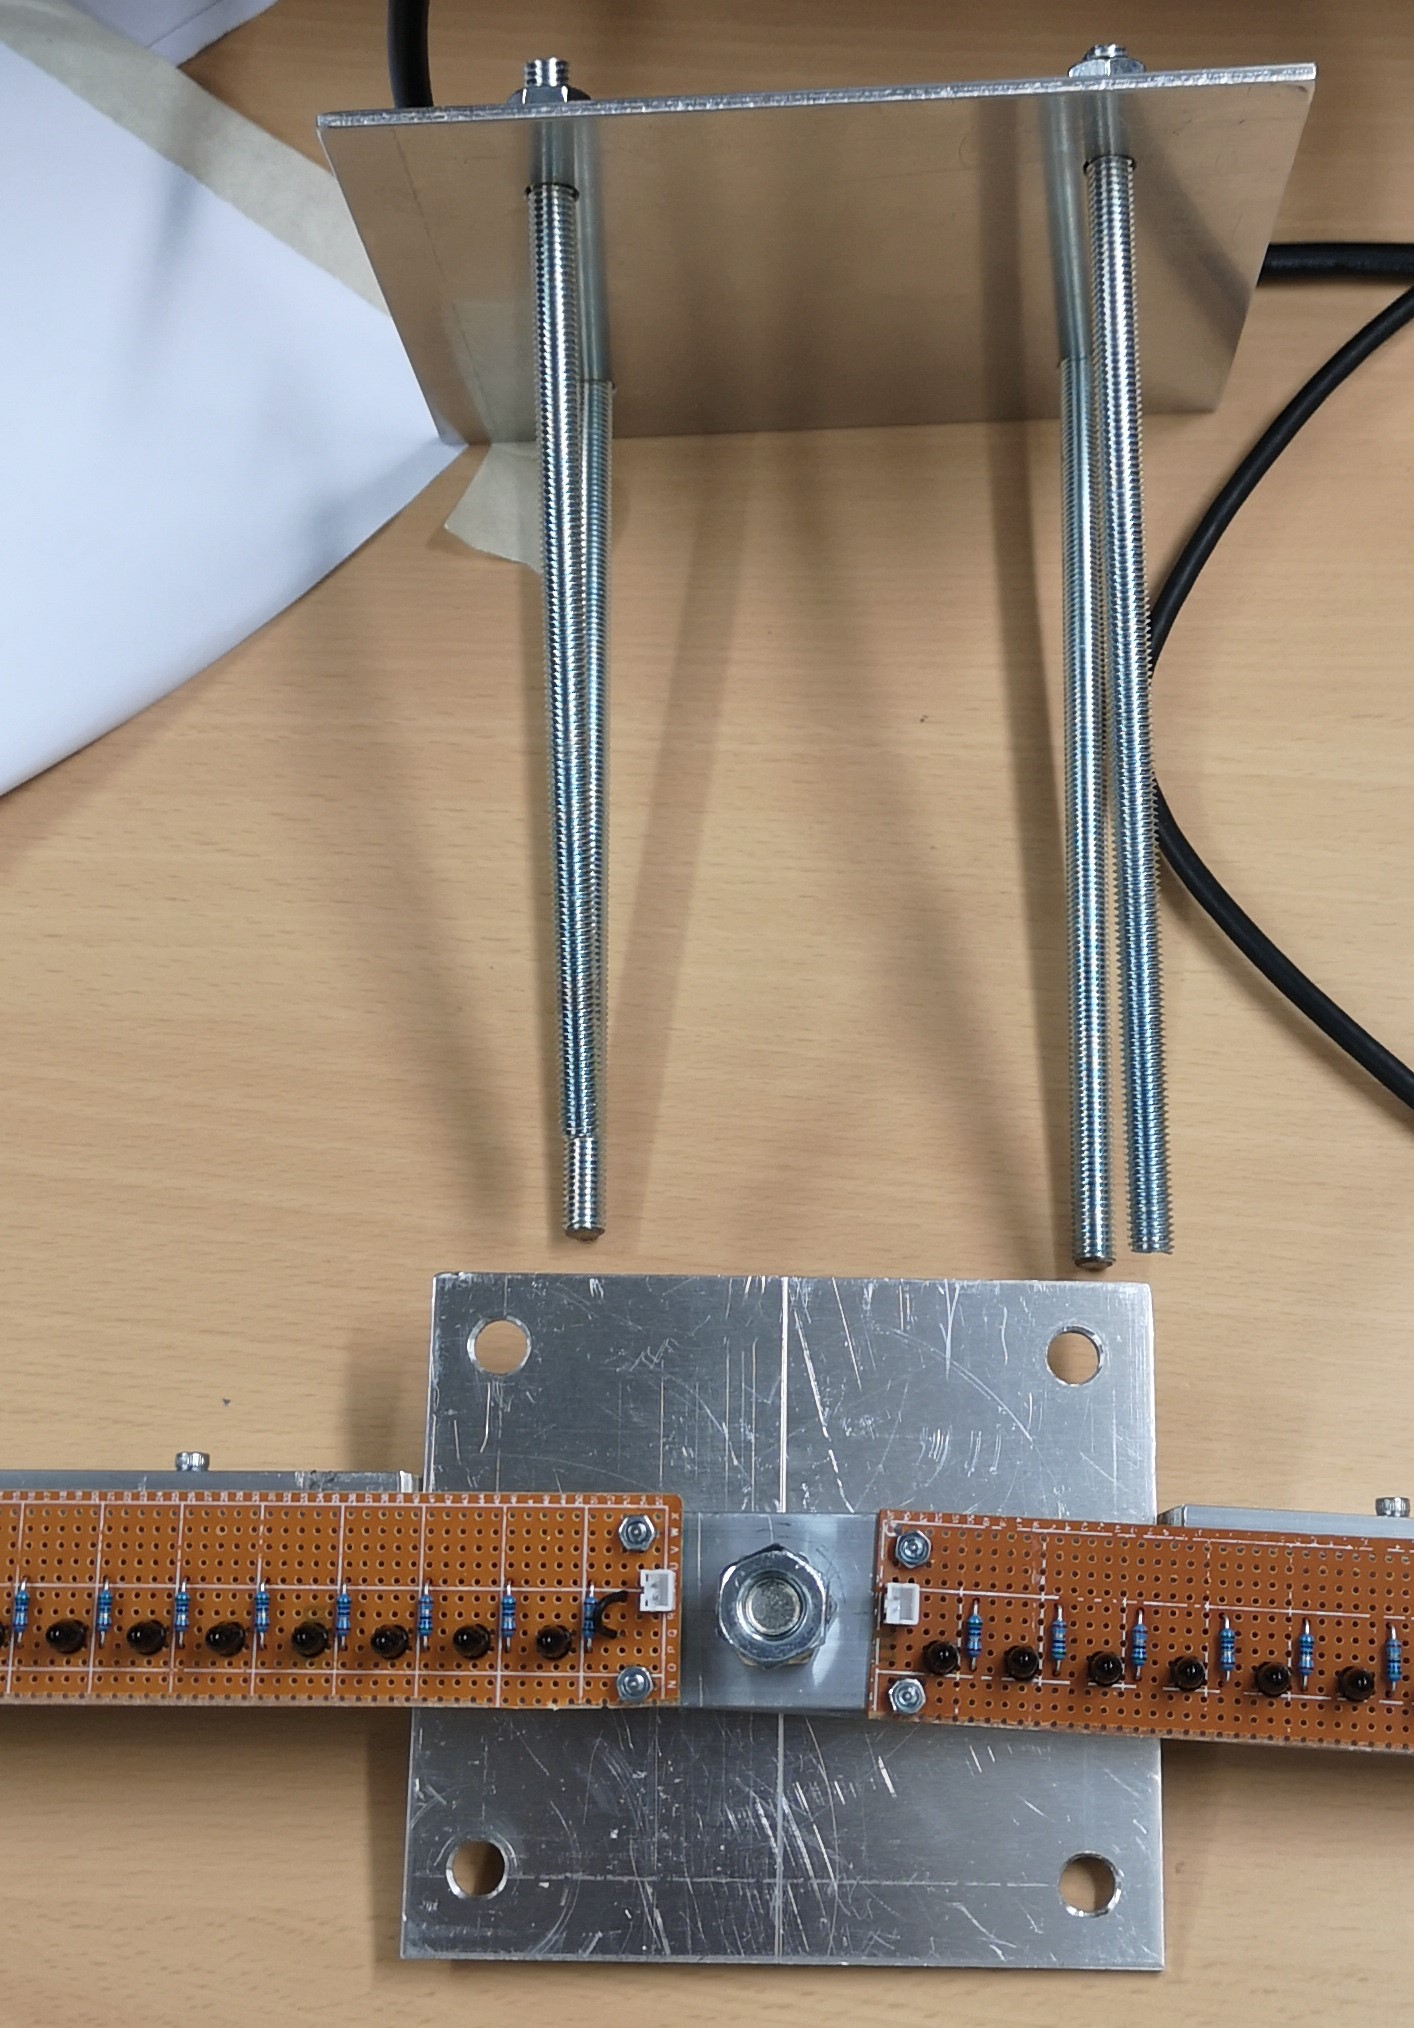
\includegraphics[height=13cm]{assets/figures/fixation_eclairage1.PNG}
    \caption{Fixation leds 1}
\end{figure}

\begin{figure}[H]
    \centering
    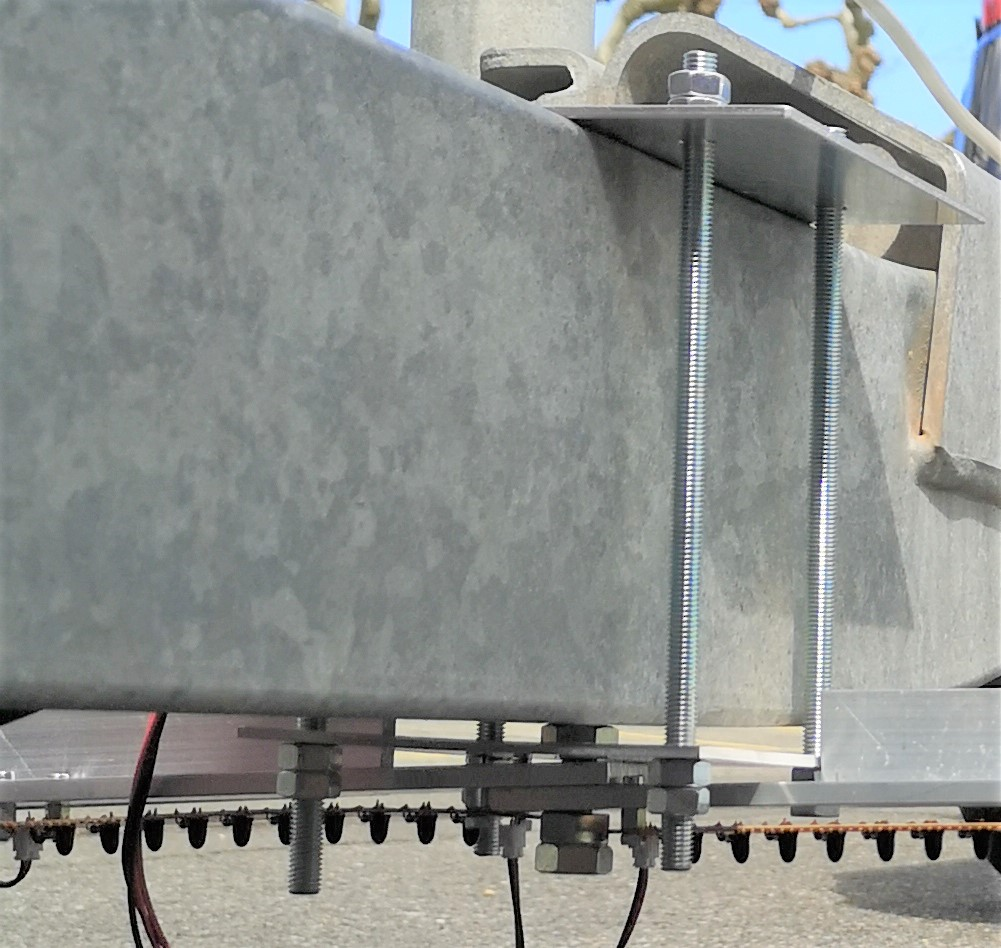
\includegraphics[width=11cm]{assets/figures/fixation_eclairage2.PNG}
    \caption{Fixation leds 2}
\end{figure}

Après essai entre 5 et 10 km/h sur le parking de l'école (surface pas forcément très régulière), la fixation reste en place et grâce à la structure du rails de leds, le tout vibre très peu.
\subsection{Boitier}
Ci-dessous la disposition des éléments du boitier:

\begin{figure}[H]
    \centering
    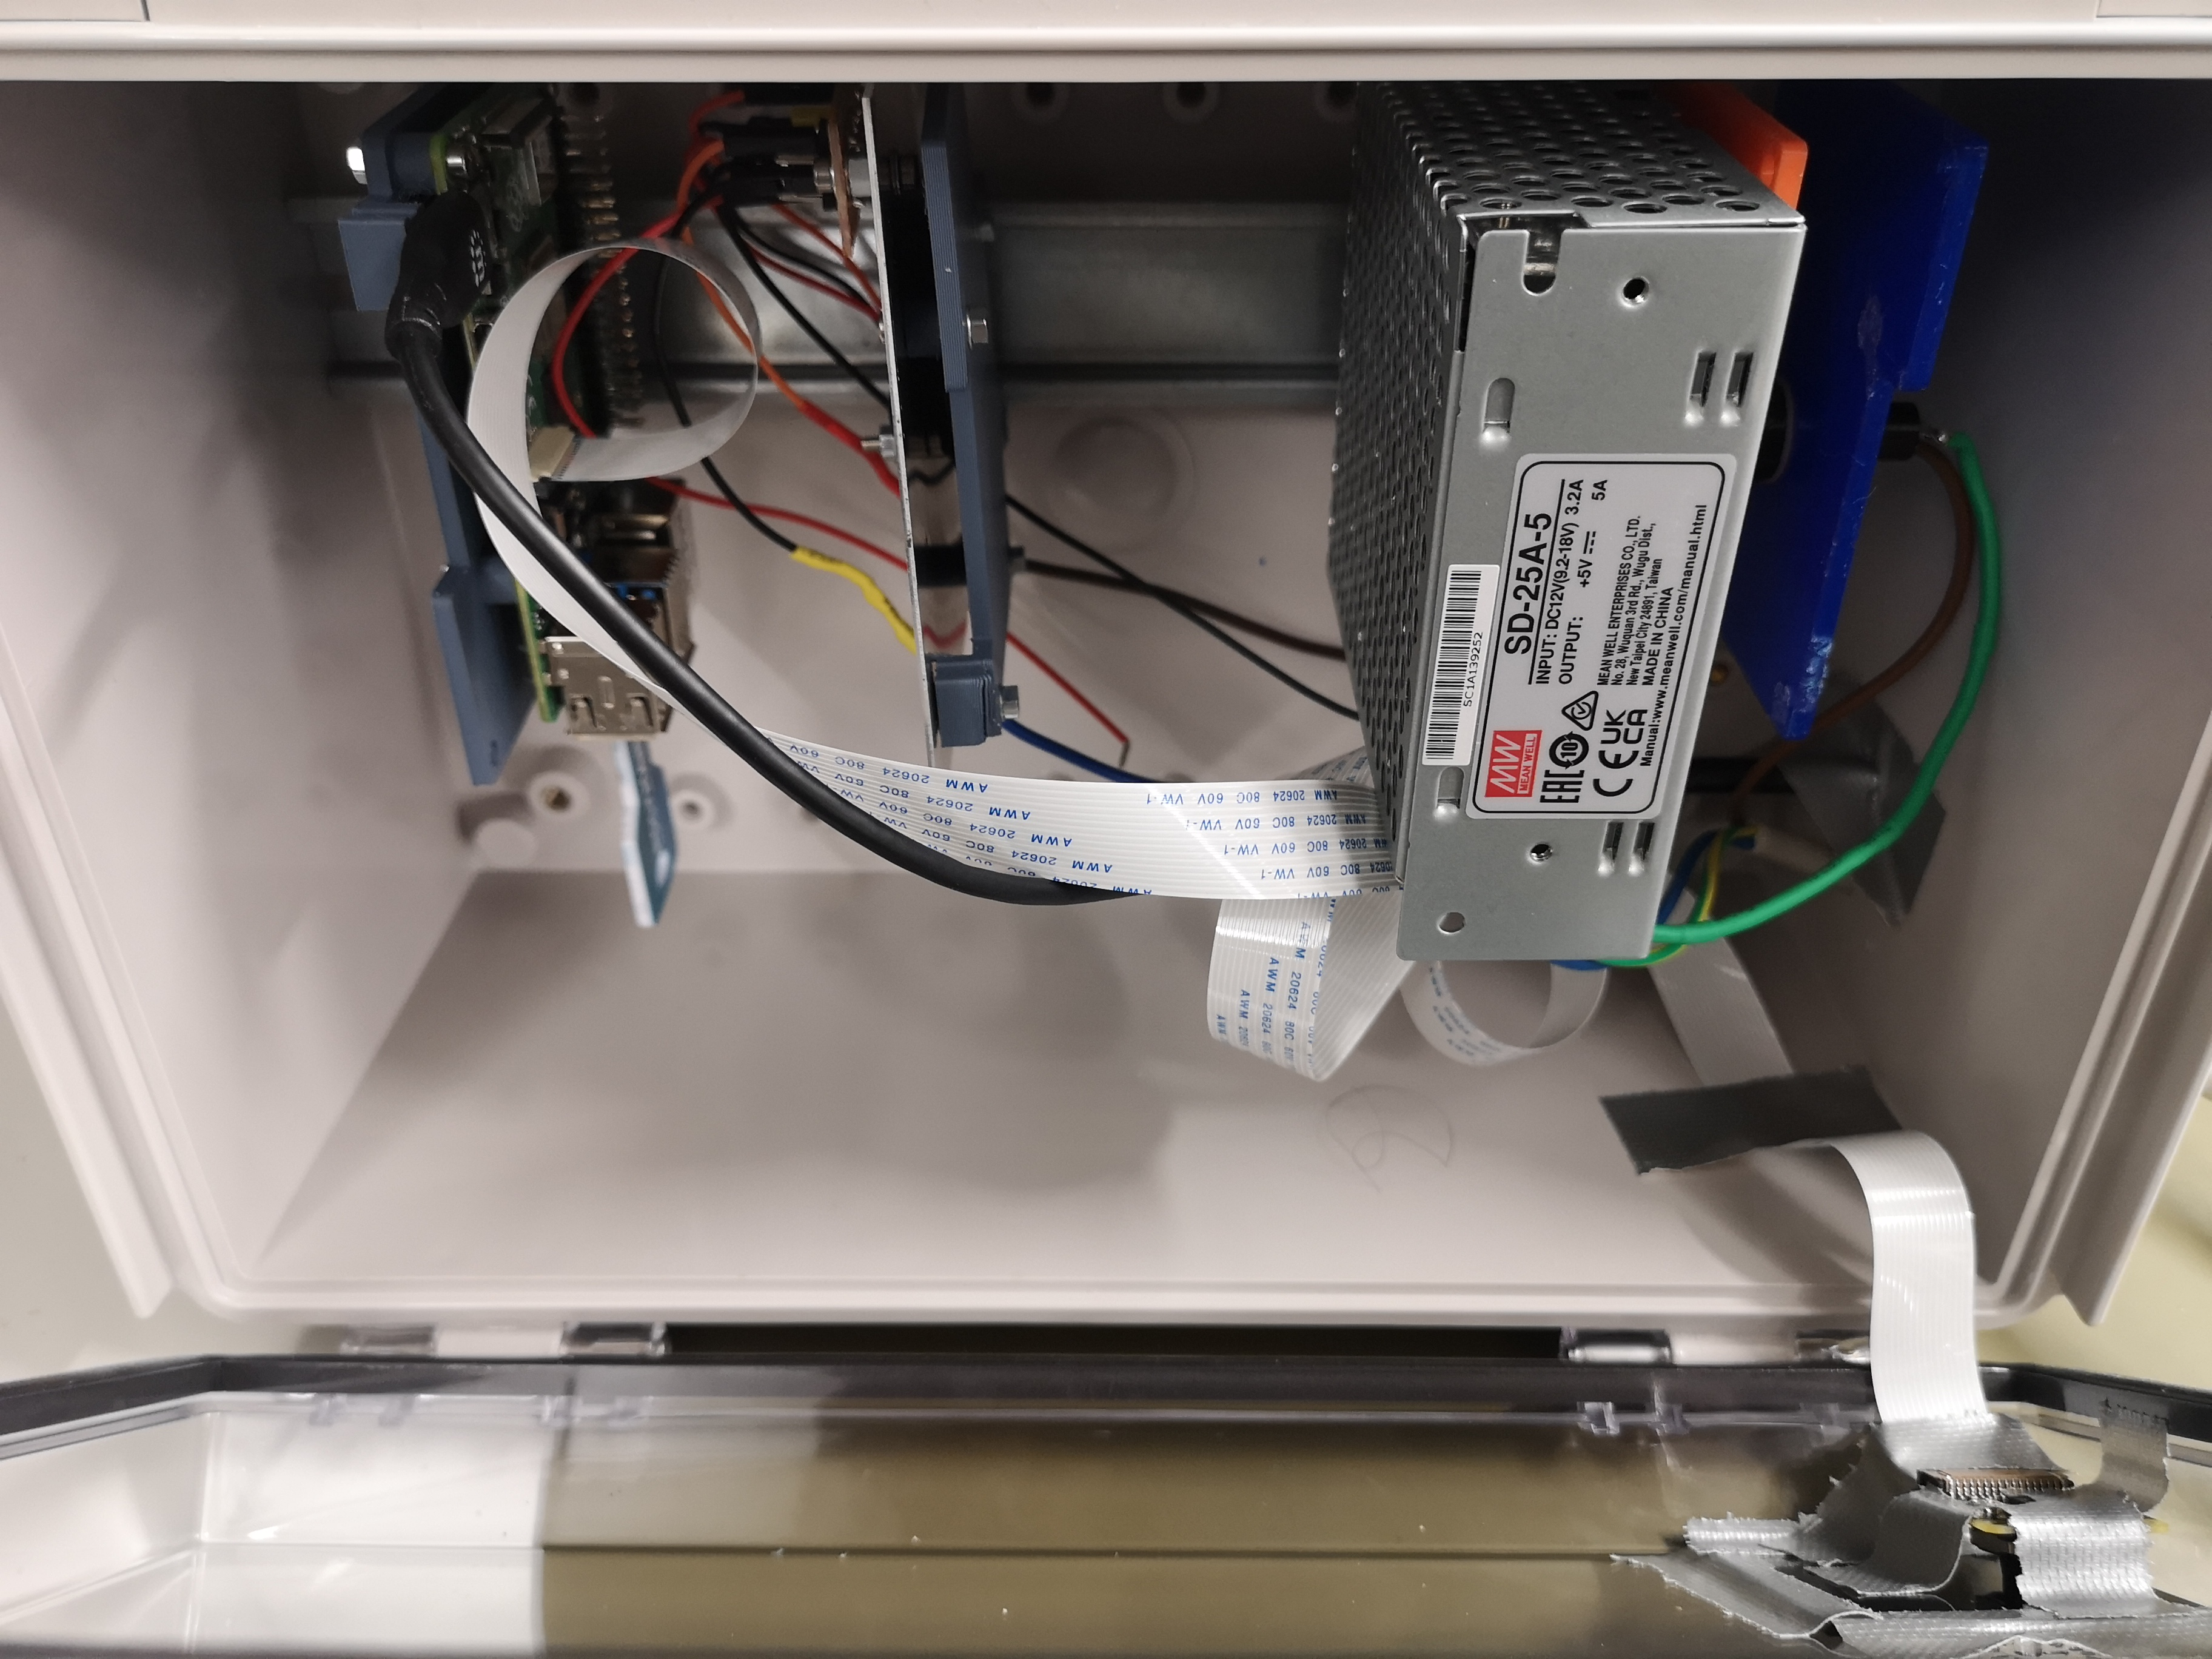
\includegraphics[width=11cm]{assets/figures/boitier_montage.jpg}
    \caption{Fixation dans le boitier}
\end{figure}

De gauche à droite, on retrouve le Rpi4, le régulateur 1.5 V, l'alimentation 5 V, le fusible d'entrée et,
en bas à droite, la caméra équipée de son filtre. Ces élements sont montés sur le rail DIN dont les supports ont été imprimés
en 3D, inspirés du modèle suivant: \cite{support_Rpi_3D}.

Ci-dessous, le boitier est fixé à sa plaque d'adaptation, elle-même fixée au support du semoir.

\begin{figure}[H]
    \centering
    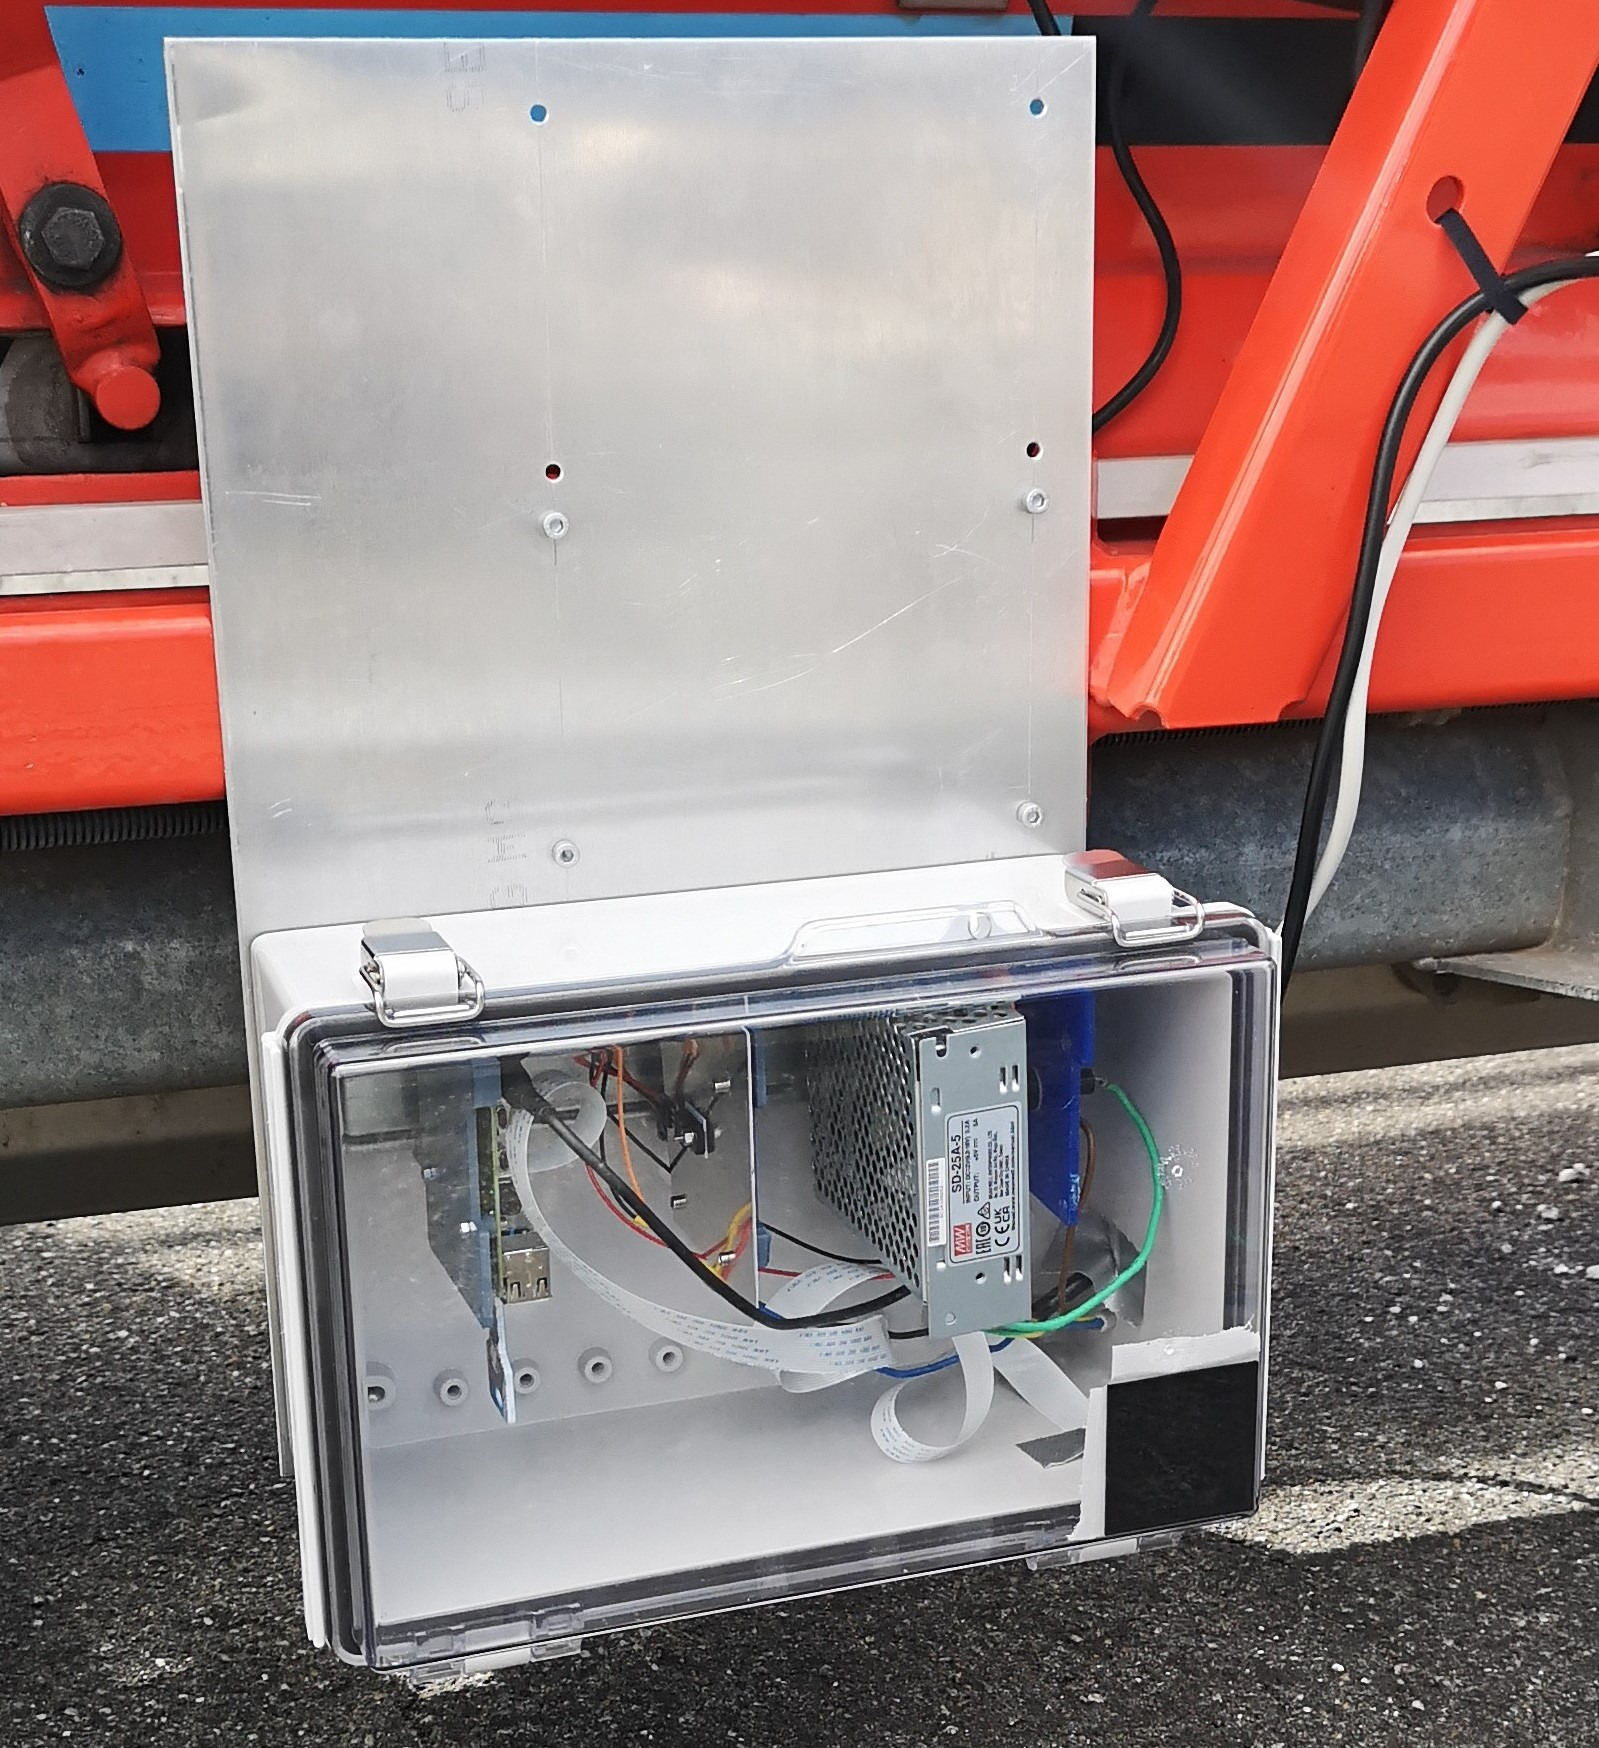
\includegraphics[height=10cm]{assets/figures/boitier_adaptation.jpg}
    \caption{Fixation sur le semoir}
\end{figure}

\subsection{Vue globale}
Ci-dessous un aperçu de l'installation globale comprenant le boitier et son support, l'éclairage et sa fixation ainsi que les câbles d'alimentations.
\begin{figure}[H]
    \centering
    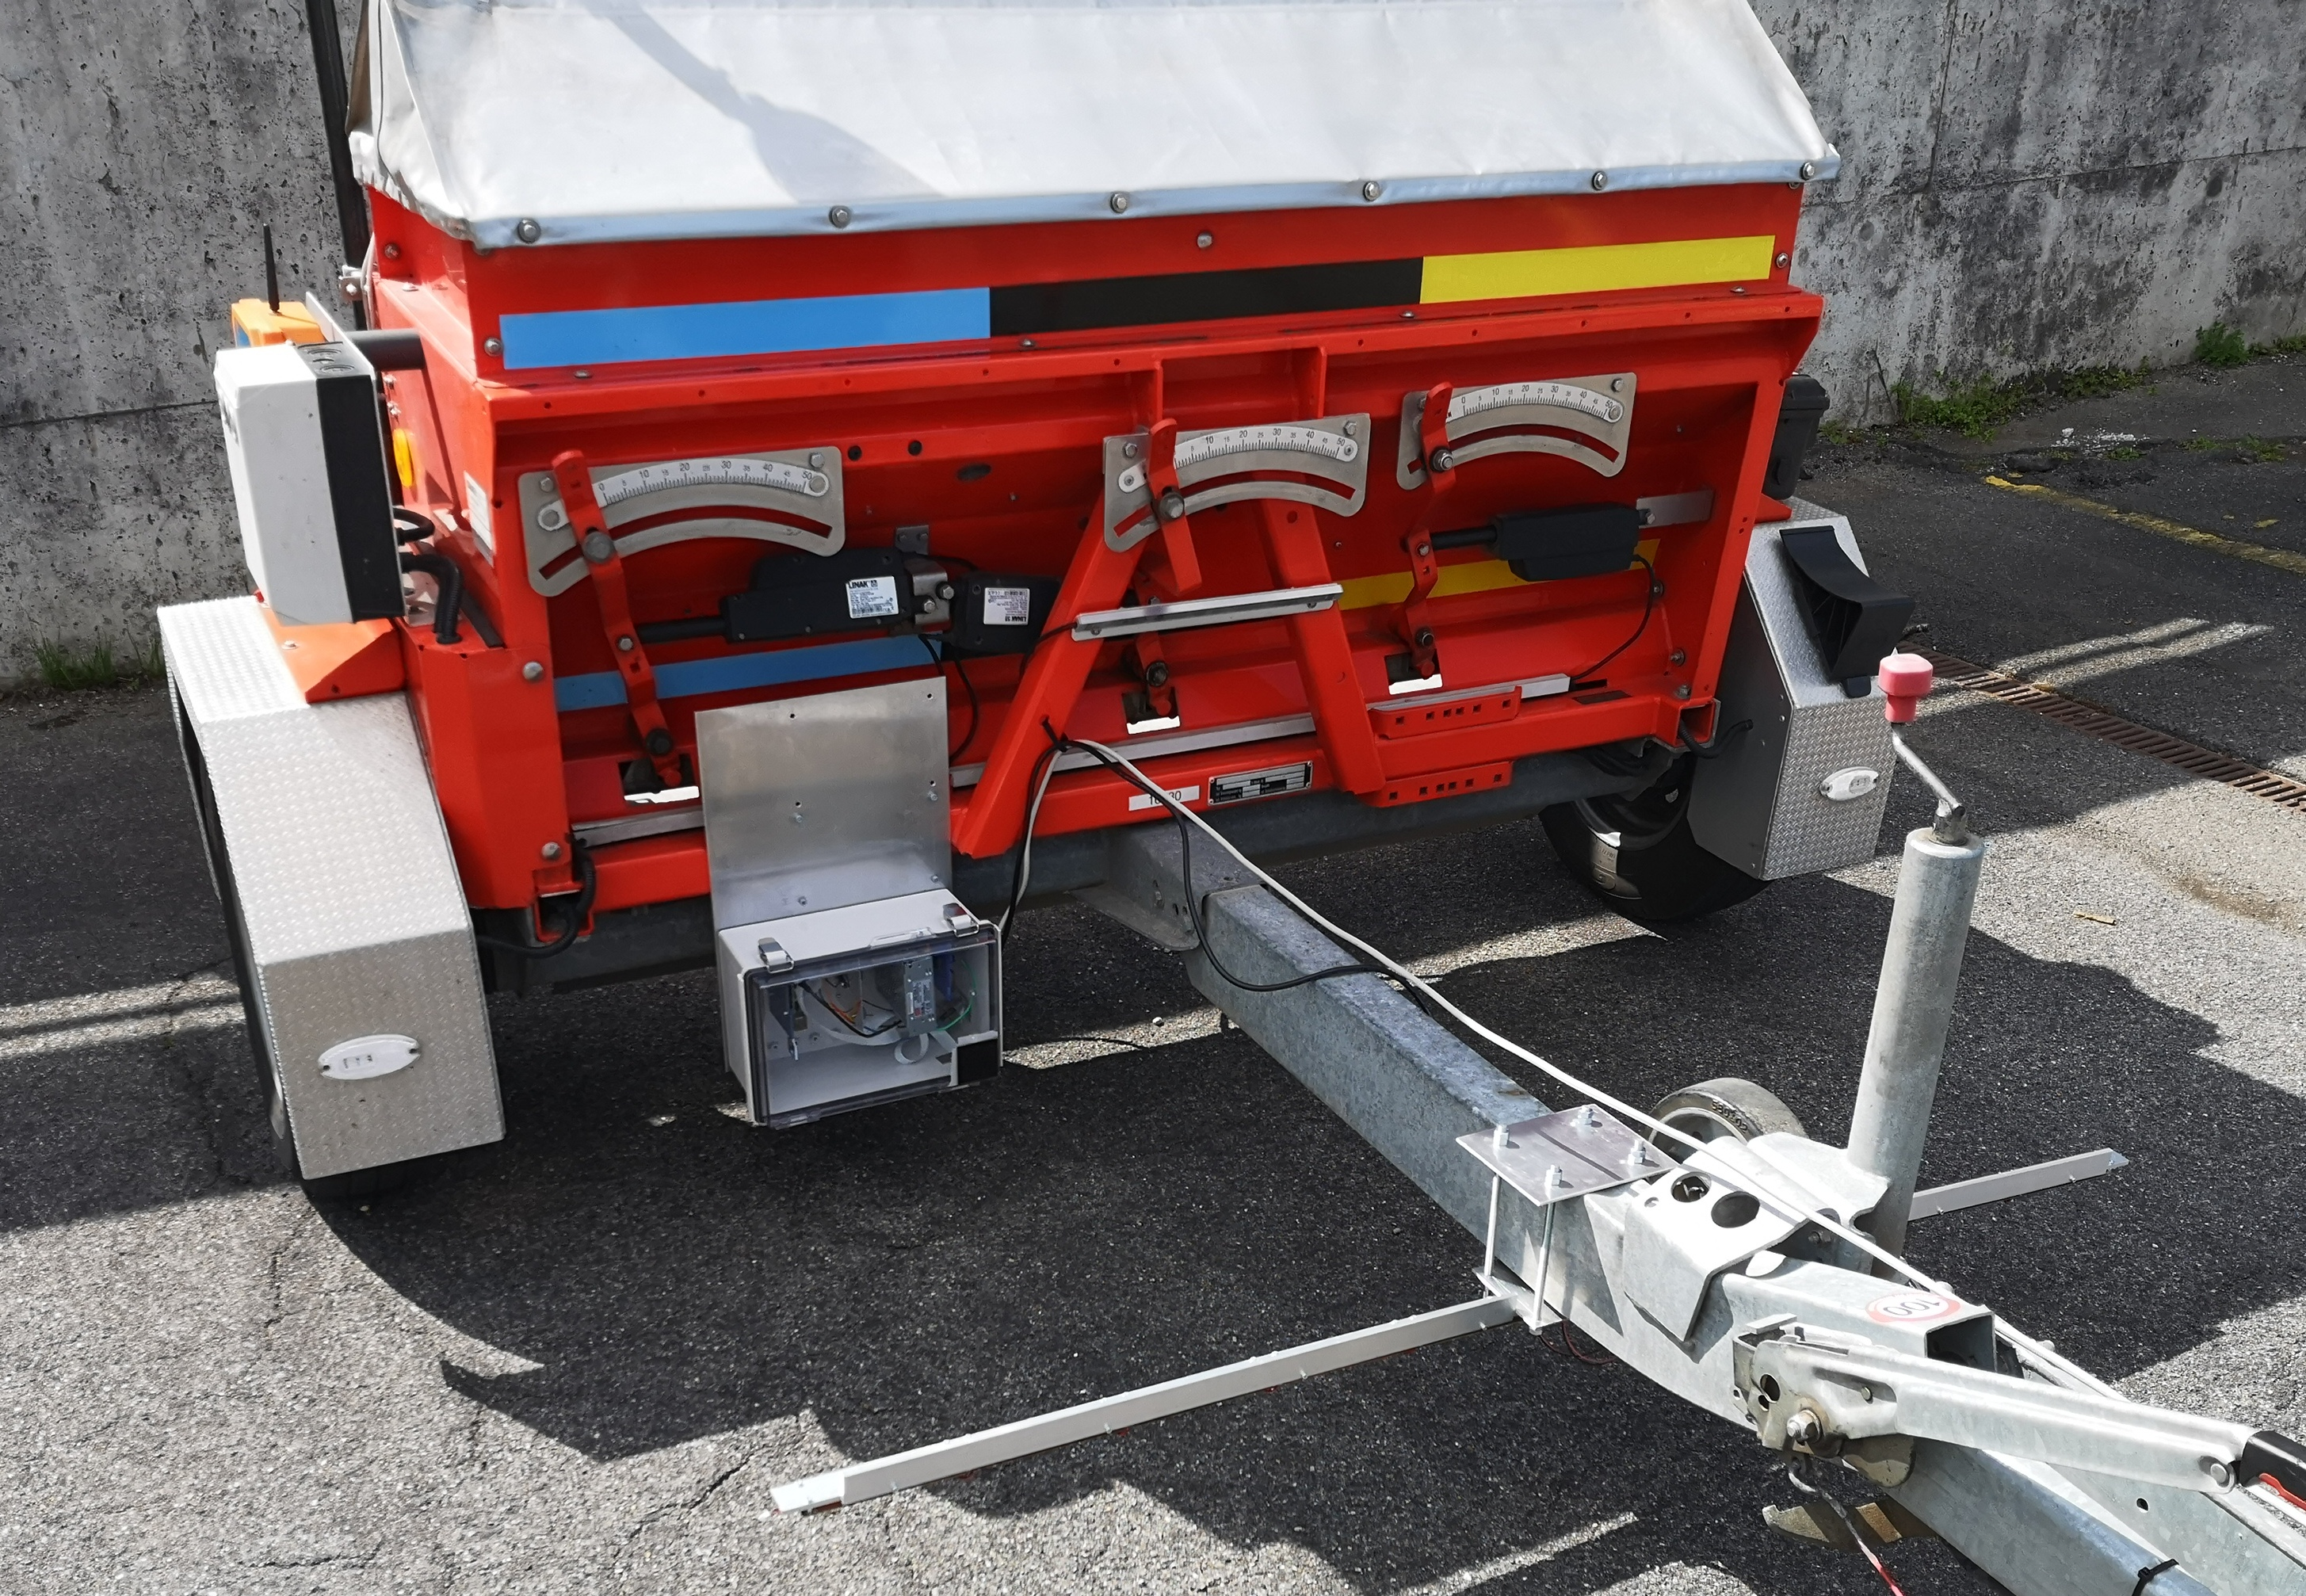
\includegraphics[height=10cm]{assets/figures/installation_globale.jpg}
    \caption{Installation entière}
\end{figure}